\documentclass[journal]{IEEEtran}

\usepackage{amsmath,amssymb}
\usepackage{booktabs}
\usepackage{graphicx}
\usepackage{xurl}

\graphicspath{{../figures/}{../../manuscript_v2_3r/displays/figures/}}
\emergencystretch=2em

\title{Projection-Selected Multidimensional Candan Refinement after FFT Tensor Support Selection}

\author{Yuhui Liu and Hangcheng Han%
\thanks{Yuhui Liu and Hangcheng Han are with the School of Integrated Circuits and Electronics, Beijing Institute of Technology, Beijing, China (e-mail: adonis3583@gmail.com; hanhangcheng@bit.edu.cn).}%
\thanks{Corresponding author: Hangcheng Han.}%
}

\begin{document}
\maketitle
\bstctlcite{BSTcontrol}

\begin{abstract}
A multidimensional fast Fourier transform (FFT) followed by top-$L$ selection gives explicit coarse neighborhoods for sparse MIMO-OFDM estimation, while physical coordinates remain off grid. We develop a non-iterative refinement that applies Candan's finite-length-corrected complex three-sample update along every active tensor axis and refits all amplitudes jointly. A calibration-free projection rule returns the refined result whenever its fitted subspace captures at least as much received energy as the grid subspace. The update reads exactly $3DL$ complex FFT samples for $D$ axes and $L$ neighborhoods. We prove that separability reduces every isolated axis triplet exactly to the one-dimensional Candan quotient, then bound multi-component interference and Gaussian noise through explicit Dirichlet-coherence, dynamic-range, SNR, and joint-fit terms. On 1200 common three-dimensional scenes, the local Candan stage improves measurement normalized mean-square error by 24.26 dB at 11.07 ms; the complete projection-selected estimator costs 11.24 ms, only 1.57\% more. The local gain remains 14.45 dB over the complete $[-0.49,0.49]$ fractional-bin interval and is positive in all 48 controlled separation--near--far cells. On 9000 clustered-delay-line tests, projection selection raises aggregate gain from 5.14 to 5.28 dB and CDL-D gain from 0.28 to 0.71 dB. Aggregate delay RMSE falls from 428.45 to 413.52 ns and joint quarter-bin accuracy rises from 7.46\% to 18.84\%.
\end{abstract}

\begin{IEEEkeywords}
MIMO-OFDM, off-grid estimation, DFT interpolation, projection selection, FFT tensor estimation, channel estimation.
\end{IEEEkeywords}

\section{Introduction}

MIMO-OFDM observations organize a small number of propagation components across array, frequency, and slow-time dimensions. Tensor models preserve this multidomain coupling and return explicit angle--delay--Doppler coordinates together with complex amplitudes, which is useful for both channel reconstruction and physical-parameter processing \cite{sidiropoulos2000parallel,kolda2009tensor,qian2018tensor_dual_polarized,kofidis2020tensor_multicarrier,gong2023esprit_tensor_train,wang2024irs_nlos_ofdm}. A multidimensional fast Fourier transform (FFT) provides an especially short support interface: its largest coefficients identify a small set of candidate neighborhoods before a joint least-squares (LS) fit.

The same grid that makes this interface inexpensive also limits its local accuracy. Angles, delays, and Dopplers are continuous, while FFT support lies on integer bins. Globally oversampled dictionaries reduce this mismatch at the cost of a larger and more coherent search space. Gridless covariance fitting, atomic-norm recovery, sparse Bayesian learning (SBL), and Newtonized pursuit remove the grid more directly, but require iterative support or continuous-coordinate optimization \cite{stoica2011spice,yang2013ogsbi,mamandipoor2016nomp,wu2023gridless_multifrequency,pote2023ml_gridless,wu2024nonuniform_gridless,wu2024coffee,pote2025lws_sbl}. Recent estimators exploit Kronecker structure, tensor decompositions, or efficient Bayesian updates rather than enlarging a generic search budget \cite{he2025offgrid_kronecker,chen2025structured_tensor_fdd,dealmeida2025bdris_tensor,cao2026offgrid_tucker,moderl2025fast_bsbl}.

Three-sample DFT interpolation offers a complementary operating point. Candan's finite-length-corrected complex ratio estimates a fractional frequency from a peak and its two neighbors \cite{candan2011three_dft}. It is closed form and highly accurate for an isolated tone, yet its use after multidimensional top-$L$ selection raises two receiver-level questions: how perturbations in a selected tensor neighborhood propagate through the complex quotient, and whether the resulting joint fit should replace the grid fit under multipath and channel-model mismatch. These questions are not answered by treating the one-dimensional interpolator as an unconditional post-processing step.

We address both questions with a projection-selected multidimensional Candan estimator. One FFT selects $L$ neighborhoods. Along every active axis, the estimator reads the center coefficient and its two periodic neighbors, applies the finite-length correction, clips the fractional step to one half bin, and refits all amplitudes jointly. A receiver-observable rule returns the candidate whose fitted subspace captures more received energy, so the projection principle sets the decision point directly. The local update uses $3DL$ complex FFT samples in a fixed-cost closed-form path.

The evidence consistently favors this design. On 1200 common three-dimensional scenes, the local Candan stage improves measurement NMSE by 24.26 dB at 11.07 ms, compared with 7.30 dB for a $125L$ Cartesian local search and 2.28 dB for one fixed-support Newton step. Projection selection takes 11.24 ms, a 1.57\% increment, and returns the same reconstruction throughout this campaign. The local gain remains 14.45 dB when offsets span the complete $[-0.49,0.49]$ interval and averages 10.46 dB across 48 controlled separation--near--far cells. On 9000 clustered-delay-line (CDL) tests, projection selection raises aggregate gain from 5.14 to 5.28 dB and CDL-D gain from 0.28 to 0.71 dB. It also improves aggregate delay RMSE and fine joint-coordinate accuracy.

The paper makes three contributions:
\begin{enumerate}
  \item It specifies a complete non-iterative estimator from FFT top-$L$ support through axis-wise complex three-sample correction, periodic alias handling, joint LS, and calibration-free projection selection. Orthonormal grid atoms and the refined QR factor reduce selection to fitted-energy comparisons.
  \item It proves the exact isolated tensor-to-scalar Candan reduction and gives a high-probability quotient bound with explicit aperture, separation, dynamic-range, sparsity, and SNR dependence. A steering-Jacobian result carries coordinate error into the joint fit.
  \item It validates accuracy, runtime, full-offset behavior, 48-cell controlled stress, CDL channel and physical-parameter accuracy, and reproducibility on disjoint seeds. The released per-scene results and MATLAB figure sources support independent reproduction.
\end{enumerate}

\section{Related Work}

\emph{FFT support and local interpolation:} Matching pursuit, orthogonal matching pursuit (OMP), and multiple-measurement-vector recovery produce explicit supports through correlation and coefficient updates \cite{mallat1993matching,pati1993omp,tropp2007omp,cotter2005mmv}. An FFT top-$L$ front end is shorter: it selects distinct spectral peaks once and then performs a joint fit. Classical Fourier-coefficient interpolation includes Quinn's estimator, while Candan provides the finite-length-corrected three-sample update executed here \cite{quinn1994fourier_interpolation,candan2011three_dft}. We apply that update independently along every tensor axis and add a fitted-subspace decision after joint LS.

\emph{Continuous sparse estimation:} Off-grid SBL perturbs dictionary parameters, Newtonized OMP repeatedly refines detected components, and gridless covariance or atomic-norm methods recover continuous spectra through structured optimization \cite{yang2013ogsbi,mamandipoor2016nomp,stoica2011spice,wagner2021gridless_nua,wu2023gridless_multifrequency,pote2023ml_gridless,wu2024nonuniform_gridless,wu2024coffee}. Recent routes include inversion-free, light-weight sequential, and fast variational SBL \cite{song2024inversion_free_sbl,pote2025lws_sbl,moderl2025fast_bsbl}. Efficient off-grid Bayesian estimation also exploits Kronecker-structured signals directly \cite{he2025offgrid_kronecker}. These algorithms revise a global support or latent model, whereas the proposed estimator provides a fixed-cost closed-form refinement when an FFT neighborhood list is already available.

\emph{Tensor and structured channel estimation:} Tensor methods exploit multilinear coupling, Vandermonde factors, and identifiable low-rank structure in massive MIMO, multicarrier estimation, MIMO radar, and RIS channels \cite{qian2018tensor_dual_polarized,kofidis2020tensor_multicarrier,xu2022tensor_mimo_radar,gong2023esprit_tensor_train,du2023ris_tensor_phase_noise,wang2024irs_nlos_ofdm}. Recent TSP work uses structured tensor decomposition for RIS and FDD channel estimation, including off-grid near-field Tucker models \cite{dealmeida2025bdris_tensor,chen2025structured_tensor_fdd,cao2026offgrid_tucker}. Our tensor structure enters at a different point: Proposition~1 shows that separability lets one multidimensional FFT supply exact scalar Candan triplets, after which one joint design matrix refits the selected components.

\begin{table*}[t]
\centering
\caption{Estimator contracts near the proposed operating point. ``Fixed'' denotes work independent of a convergence tolerance.}
\label{tab:closest_work}
\scriptsize
\setlength{\tabcolsep}{2.8pt}
\begin{tabular}{p{0.20\linewidth}ccp{0.18\linewidth}p{0.18\linewidth}p{0.20\linewidth}}
\toprule
Route & Support changed? & Fixed work? & Local update & Coefficient fit & Return rule \\
\midrule
FFT top-$L$ & No & Yes & none & one grid LS & grid estimate \\
Quadratic power interpolation & No & Yes & $3DL$ power samples & one final LS & local estimate \\
Candan \cite{candan2011three_dft} & No & Yes & $3DL$ complex samples & one final LS & local estimate \\
Cartesian local search & No & Yes & prescribed $5^D L$ scores & one final LS & local estimate \\
One-step fixed-support Newton & No & Yes & one derivative step & one final LS & local estimate \\
NOMP \cite{mamandipoor2016nomp} & Yes & No & repeated Newton updates & repeated & convergence/CFAR estimate \\
Gridless/SBL \cite{wu2023gridless_multifrequency,pote2025lws_sbl} & Global/adaptive & No & iterative structured solver & iterative & continuous estimate \\
Proposed & No & Yes & $3DL$ complex samples & joint LS; FFT grid energy & higher-energy fitted subspace \\
\bottomrule
\end{tabular}
\end{table*}

\section{Signal Model and Estimation Objective}

For tensor dimensions $N_a\times N_\tau\times N_\nu$, the synthetic observation is
\begin{equation}
 \mathcal{Y}=\mathcal{Y}_0+\mathcal{W}
 =\sum_{\ell=1}^{L}\beta_\ell\,
 \mathbf{a}_{N_a}(b_{a,\ell})\circ
 \mathbf{a}_{N_\tau}(b_{\tau,\ell})\circ
 \mathbf{a}_{N_\nu}(b_{\nu,\ell})+\mathcal{W},
 \label{eq:observation_model}
\end{equation}
where $\beta_\ell\in\mathbb{C}$, $\circ$ is the outer product, and
\begin{equation}
 [\mathbf{a}_{N}(b)]_n=N^{-1/2}\exp\!\left(j2\pi nb/N\right),
 \quad n=0,\ldots,N-1.
 \label{eq:steering_atom}
\end{equation}
Each coordinate is $b_{d,\ell}=k_{d,\ell}+\delta_{d,\ell}$, where $k_{d,\ell}$ is the nearest periodic dictionary index and $\delta_{d,\ell}\in[-1/2,1/2)$ is its fractional offset. The executed front end forms the orthonormal multidimensional FFT
\begin{equation}
 \mathcal{Z}=\mathcal{F}_{N_a,N_\tau,N_\nu}\{\mathcal{Y}\},
 \qquad
 \mathcal{S}_0=\operatorname{Top}_{L}\{|\mathcal{Z}[\mathbf{k}]|\},
 \label{eq:fft_top_l}
\end{equation}
where $\operatorname{Top}_{L}$ returns $L$ distinct bins in descending magnitude. A single pass selects the known number $L$ of periodic neighborhoods, within which the estimator refines the coordinates and amplitudes.

Define the normalized complex Dirichlet kernel
\begin{equation}
 g_N(x)=\frac{1}{N}\sum_{n=0}^{N-1}e^{j2\pi nx/N}
 =e^{j\pi(N-1)x/N}\frac{\sin(\pi x)}{N\sin(\pi x/N)},
 \label{eq:complex_dirichlet}
\end{equation}
with its continuous value at integer multiples of $N$, and let
$\mu_N(x)=|g_N(x)|$. Under the unitary FFT convention, a normalized separable
atom contributes
\begin{equation}
 \left\langle\bigotimes_{r=1}^{D}\mathbf a_{N_r}(k_r),
 \bigotimes_{r=1}^{D}\mathbf a_{N_r}(b_r)\right\rangle
 =\prod_{r=1}^{D}g_{N_r}(b_r-k_r).
 \label{eq:tensor_fft_factor}
\end{equation}
Coordinate differences are interpreted periodically.

\begin{figure*}[t]
  \centering
  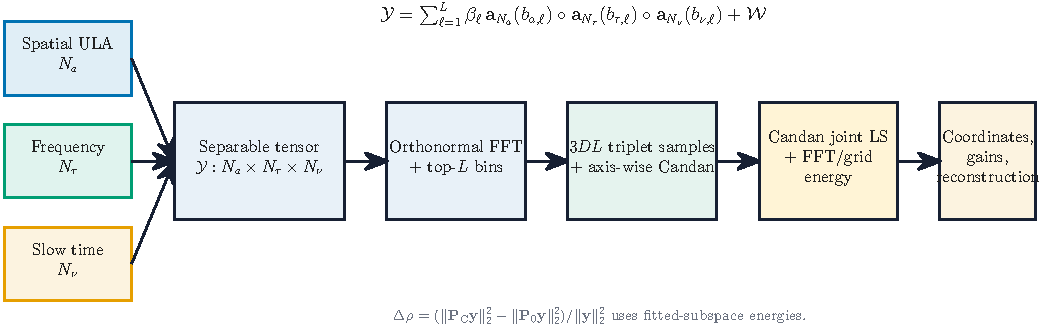
\includegraphics[width=0.96\textwidth]{tsp_system_model.pdf}
  \caption{Executed tensor-estimation interface. An orthonormal FFT selects $L$ neighborhoods; $3DL$ center/neighbor samples drive the axis-wise Candan update, and fitted-subspace energies select between the grid and Candan joint-LS outputs. The CDL experiment specializes the interface to frequency and the BS transmit-ULA dimension.}
  \label{fig:system_model}
\end{figure*}

The CDL experiment is generated separately from a 3GPP channel impulse response (CIR) using Sionna \cite{3gpp38901,hoydis2023sionna}. Let $h_{m,p}$ and $\tau_p$ be the complex response at base-station ULA element $m$ and delay of CIR component $p$. After channel normalization, the frequency--array observation is
\begin{equation}
 \begin{aligned}
 H[n,m]&=c\sum_{p=1}^{L_{\rm CIR}}h_{m,p}
 \exp(-j2\pi f_n\tau_p),\\
 Y_{\rm CDL}[n,m]&=H[n,m]+W[n,m],
 \end{aligned}
 \label{eq:cdl_observation}
\end{equation}
where $f_n$ is the baseband subcarrier frequency and $c$ is the normalization applied by the channel generator. The array dimension is the four-element base-station transmit ULA observed by one user-terminal receive element. Complex AWGN is added after CIR-to-OFDM conversion, and the resulting dense $64\times4$ channel tensor is the estimator input, giving a direct channel-domain test of parameter estimation.

The main reconstruction metric is measurement-domain normalized mean-square error (NMSE),
\begin{equation}
 \operatorname{NMSE}_{\mathrm{dB}}=10\log_{10}
 \frac{\|\widehat{\mathcal{Y}}-\mathcal{Y}_0\|_F^2}
 {\|\mathcal{Y}_0\|_F^2}.
 \label{eq:nmse_metric}
\end{equation}
For method $m$, the reported reconstruction gain is $G_m=\operatorname{NMSE}_{\rm grid,dB}-\operatorname{NMSE}_{m,\rm dB}$, so a positive value favors $m$. Parameter errors use minimum-cost Hungarian assignment and circular distance on every active FFT axis. The all-axis $q$-bin accuracy is the fraction of matched components whose absolute circular error is at most $q$ bin on every active axis; we report $q\in\{0.1,0.25,0.5\}$ as tenth-, quarter-, and half-bin accuracy.

For CDL physical metrics, the reference set retains the $\min(L,L_{\rm CIR})$ CIR components with largest summed array power as individual paths. Delay truth is $\tau_p$. A half-wavelength one-dimensional ULA identifies projected spatial frequency, whose reference is the peak of a 4096-point FFT of each clean per-component array response. Estimated bins are converted to delay and projected spatial frequency, then assigned by squared errors normalized to the delay and spatial bin resolutions. The reported projected-angle error is the minimum broadside-angle error over valid ULA aliases. This fixes reference selection, weighting, assignment, and alias handling before evaluation.

\begin{table}[t]
\centering
\caption{Scene-generation and channel-observation protocol.}
\label{tab:system_params}
\footnotesize
\setlength{\tabcolsep}{3pt}
\begin{tabular}{@{}p{0.36\columnwidth}p{0.56\columnwidth}@{}}
\toprule
Item & Executed setting \\
\midrule
Synthetic tensor & $128\times16\times32$; $L\in\{2,4,8\}$ \\
Coarse support & uniform distinct flat indices; unconstrained separation \\
Offsets / gains & matched scenes: $\mathcal{U}[-0.35,0.35]$; full-offset: $\mathcal{U}[-0.49,0.49]$ bin per axis; $\mathcal{CN}(0,1)$ \\
Synthetic AWGN & $\sigma^2=P_{\mathcal{Y}_0}10^{-\mathrm{SNR}/10}$; SNR $\in\{0,10,20,30\}$ dB \\
Scene accounting & every generated scene retained in aggregate metrics \\
\midrule
CDL carrier / spacing & 60 GHz; 64 subcarriers at 120 kHz \\
CDL spatial aperture & four-element BS transmit ULA, $\lambda/2$; one UT receive element \\
Profiles / delay spread & 3GPP CDL-A/C/D; 100 ns; static terminal \\
CDL counts / SNR & $L\in\{4,8,16\}$; $\{0,10,20,30\}$ dB \\
CDL test split & 5 seeds; 50 channels/profile/seed; higher fitted-energy return rule \\
\bottomrule
\end{tabular}
\end{table}

\section{Projection-Selected Multidimensional Candan Refinement}

The proposed estimator preserves the $L$ neighborhoods selected by \eqref{eq:fft_top_l}. It applies a closed-form complex three-sample correction along every active axis, forms one joint-LS reconstruction, and selects between the grid and Candan fitted subspaces. Figure~\ref{fig:architecture} summarizes the executed path.

\begin{figure*}[t]
  \centering
  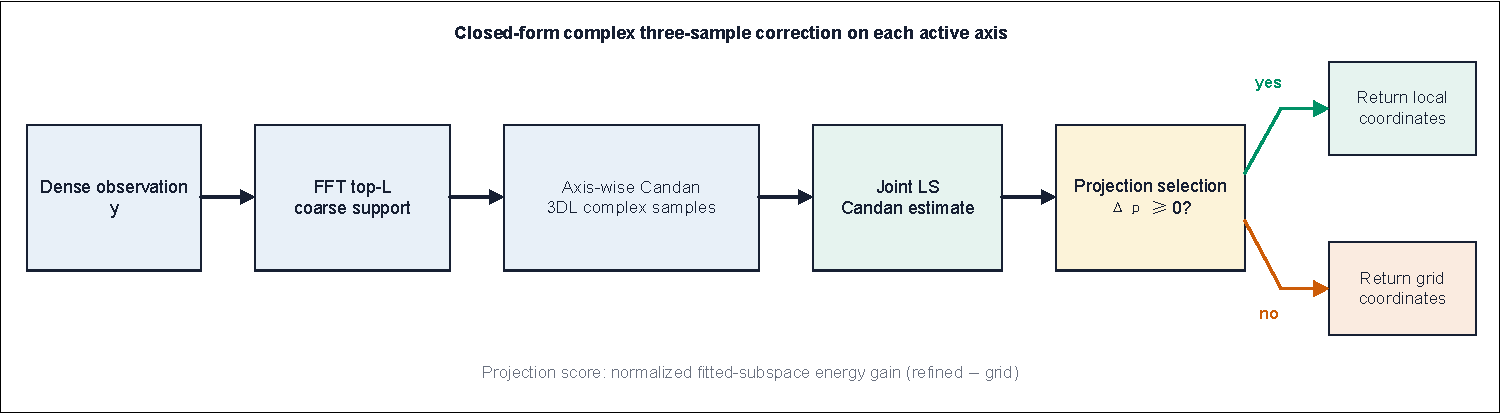
\includegraphics[width=0.96\textwidth]{tsp_method_flow.pdf}
  \caption{Projection-selected multidimensional Candan refinement. One FFT supplies $3DL$ triplet samples. The grid energy comes directly from the selected orthonormal FFT coefficients, while the refined energy is obtained from the Candan design QR factor.}
  \label{fig:architecture}
\end{figure*}

\subsection{Axis-Wise Complex Three-Sample Update}

Let $\mathbf{k}_\ell=(k_{1,\ell},\ldots,k_{D,\ell})$ be a selected FFT bin. For axis $d$, denote the center coefficient and its two periodic neighbors by
\begin{equation}
 Z_{d,0}=\mathcal{Z}[\mathbf{k}_\ell],\quad
 Z_{d,-}=\mathcal{Z}[\mathbf{k}_\ell-\mathbf{e}_d],\quad
 Z_{d,+}=\mathcal{Z}[\mathbf{k}_\ell+\mathbf{e}_d],
 \label{eq:candan_triplet}
\end{equation}
where all non-$d$ coordinates remain fixed and indexing wraps modulo $N_d$. Candan's finite-length-corrected update is
\begin{equation}
 \widetilde{\delta}_{d,\ell}=
 \frac{\tan(\pi/N_d)}{\pi/N_d}
 \operatorname{Re}\!\left\{
 \frac{Z_{d,-}-Z_{d,+}}
 {2Z_{d,0}-Z_{d,-}-Z_{d,+}}
 \right\}.
 \label{eq:candan_update}
\end{equation}
The deployed coordinate is
\begin{equation}
 \widehat b_{d,\ell}=
 \operatorname{mod}_{N_d}\!\left(
 k_{d,\ell}+\operatorname{clip}(\widetilde{\delta}_{d,\ell},-1/2,1/2)
 \right).
 \label{eq:candan_clip}
\end{equation}
For the four-element CDL array, the same Nyquist-alias convention is applied to the grid and refined coordinates before evaluation.

The normalized denominator statistic used in the analysis is
\begin{equation}
 \zeta_{d,\ell}=
 \frac{|2Z_{d,0}-Z_{d,-}-Z_{d,+}|}
 {|Z_{d,-}|+2|Z_{d,0}|+|Z_{d,+}|+\varepsilon}.
 \label{eq:candan_stability}
\end{equation}
where $\varepsilon$ is machine precision. This statistic lies in $[0,1]$, is computed directly from the received triplet, and scales the quotient perturbation bound in Section~\ref{sec:analysis}. The final return decision uses the scene-level fitted-energy statistic below.

\subsection{Joint LS and Calibration-Free Projection Selection}

Let $\mathbf y=\operatorname{vec}(\mathcal Y)$ and let $\mathbf B=[\mathbf b_1,\ldots,\mathbf b_L]\in\mathbb R^{D\times L}$ collect component coordinates. Define $\mathbf a(\mathbf b_\ell)=\bigotimes_{d=1}^{D}\mathbf a_{N_d}(b_{d,\ell})$ and $\mathbf A(\mathbf B)=[\mathbf a(\mathbf b_1),\ldots,\mathbf a(\mathbf b_L)]$. The matrices $\mathbf B_0$ and $\mathbf B_{\rm C}$ contain the selected grid and Candan coordinates. The refined amplitudes and reconstruction are
\begin{equation}
 \widehat{\boldsymbol{\beta}}_{\rm C}
 =\arg\min_{\boldsymbol{\beta}}
 \|\mathbf{y}-\mathbf{A}(\mathbf{B}_{\rm C})\boldsymbol{\beta}\|_2^2,
 \qquad
 \widehat{\mathbf{y}}_{\rm C}=\mathbf{A}(\mathbf{B}_{\rm C})
 \widehat{\boldsymbol{\beta}}_{\rm C}.
 \label{eq:ls_reconstruction}
\end{equation}
Let $\mathbf P_s=\mathbf A(\mathbf B_s)\mathbf A(\mathbf B_s)^\dagger$ for $s\in\{0,{\rm C}\}$ denote the grid and refined orthogonal projectors. The normalized residual reduction is equivalently the fitted-energy difference
\begin{equation}
 \Delta\rho=\frac{\|\mathbf P_{\rm C}\mathbf y\|_2^2-
 \|\mathbf P_0\mathbf y\|_2^2}{\|\mathbf y\|_2^2}.
 \label{eq:observable_residual}
\end{equation}
The selected integer-bin atoms are distinct columns of the unitary DFT basis, so
$\|\mathbf P_0\mathbf y\|_2^2=\sum_{\mathbf k\in\mathcal S_0}|\mathcal Z[\mathbf k]|^2$.
If $\mathbf A(\mathbf B_{\rm C})=\mathbf Q_{\rm C}\mathbf R_{\rm C}$ is the QR factorization already used for the refined LS, then
$\|\mathbf P_{\rm C}\mathbf y\|_2^2=\|\mathbf Q_{\rm C}^H\mathbf y\|_2^2$.
Thus the existing FFT coefficients and refined QR factor supply both fitted energies. The returned result is
\begin{equation}
 (\widehat{\mathbf{B}},\widehat{\mathbf{y}})=
 \begin{cases}
 (\mathbf{B}_{\rm C},\widehat{\mathbf{y}}_{\rm C}),&\Delta\rho\geq0,\\
 (\mathbf{B}_0,\mathbf P_0\mathbf y),&\Delta\rho<0.
 \end{cases}
 \label{eq:residual_gate}
\end{equation}
The decision point $\Delta\rho=0$ follows directly from returning the fitted subspace that explains more of the received tensor. Across 60 numerical identity checks, the projection and explicit-residual decisions agree within $5.44\times10^{-15}$, and QR- and reconstruction-based projection energies agree within $1.09\times10^{-14}$ after normalization.

The update reads exactly $3DL$ complex FFT samples. The complete path adds the refined joint LS and one scalar fitted-energy comparison to the common FFT top-$L$ front end.

\section{Separable Triplet Reduction and Probabilistic Error Propagation}
\label{sec:analysis}

The tensor structure reduces each isolated multidimensional triplet exactly to the scalar Candan problem. Interference and noise then enter as explicit perturbations controlled by Fourier coherence, dynamic range, and SNR.

\textbf{Proposition 1 (isolated separable triplet reduction):}
For component $\ell$, let $b_{r,\ell}=k_{r,\ell}+\delta_{r,\ell}$ with $\delta_{r,\ell}\in[-1/2,1/2]$. Without other components or noise, for axis $d$ and $q\in\{-1,0,1\}$,
\begin{equation}
\begin{aligned}
 Z^{(\ell)}[\mathbf k_\ell+q\mathbf e_d]
 &=C_{-d,\ell}g_{N_d}(\delta_{d,\ell}-q),\\
 C_{-d,\ell}&=\beta_\ell\prod_{r\ne d}g_{N_r}(\delta_{r,\ell}).
\end{aligned}
 \label{eq:isolated_triplet_factorization}
\end{equation}
The common complex factor cancels from the quotient, giving
\begin{equation}
 \frac{Z_{d,-}^{(\ell)}-Z_{d,+}^{(\ell)}}
 {2Z_{d,0}^{(\ell)}-Z_{d,-}^{(\ell)}-Z_{d,+}^{(\ell)}}
 =\frac{\tan(\pi\delta_{d,\ell}/N_d)}{\tan(\pi/N_d)}.
 \label{eq:isolated_candan_ratio}
\end{equation}
Hence the unclipped update is
\begin{equation}
 \phi_{N_d}(\delta_{d,\ell})
 =\frac{\tan(\pi\delta_{d,\ell}/N_d)}{\pi/N_d}.
 \label{eq:candan_finite_map}
\end{equation}
\emph{Proof:} Equation~\eqref{eq:tensor_fft_factor} gives the product in \eqref{eq:isolated_triplet_factorization}; changing only axis $d$ leaves all other factors unchanged. Substitution of \eqref{eq:complex_dirichlet} and the angle-addition identities yields \eqref{eq:isolated_candan_ratio}. \hfill$\square$

Thus separability removes every non-updated axis from the isolated quotient. The finite-length map retains the small bias
\begin{equation}
 b_N(\delta)=|\phi_N(\delta)-\delta|=O(N^{-2}).
 \label{eq:candan_finite_bias}
\end{equation}

\textbf{Proposition 2 (multi-component Gaussian quotient bound):}
Assume $N_d\geq3$, independent tensor noise $\mathcal{CN}(0,\sigma^2)$, and a fixed selected-bin/component association. Write
\begin{equation}
 Z_{d,q}=C_{-d,\ell}g_{N_d}(\delta_{d,\ell}-q)+u_{d,q}+w_{d,q},
 \label{eq:triplet_signal_interference_noise}
\end{equation}
where
\begin{equation}
 u_{d,q}=\sum_{j\ne\ell}\beta_j\prod_{r=1}^{D}g_{N_r}
 (b_{r,j}-k_{r,\ell}-q\mathbf 1_{\{r=d\}}).
\end{equation}
Define
\begin{equation}
 I_{d,q,\ell}=\sum_{j\ne\ell}|\beta_j|\prod_{r=1}^{D}\mu_{N_r}
 (b_{r,j}-k_{r,\ell}-q\mathbf 1_{\{r=d\}}),
 \label{eq:interference_envelope}
\end{equation}
and the target numerator, denominator, and quotient
\begin{align}
 n_{d,\ell}&=C_{-d,\ell}\{g_{N_d}(\delta+1)-g_{N_d}(\delta-1)\},\nonumber\\
 d_{d,\ell}&=C_{-d,\ell}\{2g_{N_d}(\delta)-g_{N_d}(\delta+1)-g_{N_d}(\delta-1)\},\nonumber\\
 \gamma_{d,\ell}&=n_{d,\ell}/d_{d,\ell}
 =\tan(\pi\delta/N_d)/\tan(\pi/N_d),
 \label{eq:target_num_den}
\end{align}
where $\delta=\delta_{d,\ell}$. For $\eta\in(0,1)$ let
\begin{align}
 B_{n,d,\ell}&=I_{d,-1,\ell}+I_{d,+1,\ell}
 +\sigma\sqrt{2\log(2/\eta)},\nonumber\\
 B_{d,d,\ell}&=2I_{d,0,\ell}+I_{d,-1,\ell}+I_{d,+1,\ell}
 +\sigma\sqrt{6\log(2/\eta)}.
 \label{eq:explicit_bn_bd}
\end{align}
If $B_{d,d,\ell}<|d_{d,\ell}|$, then with probability at least $1-\eta$,
\begin{equation}
\begin{aligned}
 |\widehat\delta_{d,\ell}-\delta_{d,\ell}|
 &\le b_{N_d}(\delta_{d,\ell})\\
 &\quad+c_{N_d}\frac{B_{n,d,\ell}+|\gamma_{d,\ell}|B_{d,d,\ell}}
 {|d_{d,\ell}|-B_{d,d,\ell}},\\[-1mm]
 c_N&=\frac{\tan(\pi/N)}{\pi/N}.
\end{aligned}
 \label{eq:coordinate_error_bound}
\end{equation}
\emph{Proof:} The unitary FFT preserves the noise law. Numerator noise is $\mathcal{CN}(0,2\sigma^2)$ and denominator noise is $\mathcal{CN}(0,6\sigma^2)$. Complex-Gaussian tails and a union bound give \eqref{eq:explicit_bn_bd}. The quotient identity
\begin{equation*}
 \left|\frac{n+e_n}{d+e_d}-\frac nd\right|
 \le\frac{|e_n|+|n/d||e_d|}{|d|-|e_d|}
\end{equation*}
followed by the finite-length factor and nonexpansive clipping proves \eqref{eq:coordinate_error_bound}. \hfill$\square$

The dependence is explicit. If $\Gamma_\ell=\max_{j\ne\ell}|\beta_j|/|\beta_\ell|$ and $\bar\mu_{d,q,\ell}$ is the largest coherence product in \eqref{eq:interference_envelope}, then
\begin{equation}
 I_{d,q,\ell}\le |\beta_\ell|(L-1)\Gamma_\ell\bar\mu_{d,q,\ell}.
 \label{eq:dynamic_range_interference}
\end{equation}
Under the executed SNR convention, $\sigma=\sqrt{P_{\mathcal Y_0}}10^{-\mathrm{SNR}/20}$. A simultaneous statement for all $DL$ triplets replaces $\eta$ by $\eta/(DL)$. The observable statistic $\zeta$ in \eqref{eq:candan_stability} is the measured counterpart of the denominator margin; empirically, its Spearman association with clipping is $-0.525$, $-0.508$, and $-0.506$ on CDL-A/C/D.

\textbf{Corollary 1 (propagation to the joint fit):}
Let $\mathbf A_0$ and $\widehat{\mathbf A}$ contain normalized atoms at the true and refined coordinates. If $|\widehat b_{d,\ell}-b_{d,\ell}|\le\epsilon_{d,\ell}$ periodically, define
\begin{equation}
\begin{aligned}
 \Lambda_N&=\frac{2\pi}{N}\sqrt{\frac{(N-1)(2N-1)}{6}},\\
 E_A&=\left[\sum_{\ell=1}^{L}\left(\sum_{d=1}^{D}
 \Lambda_{N_d}\epsilon_{d,\ell}\right)^2\right]^{1/2}.
\end{aligned}
 \label{eq:dictionary_lipschitz}
\end{equation}
Then $\|\mathbf A_0-\widehat{\mathbf A}\|_2\le E_A$. If $\widehat{\mathbf A}$ has full column rank,
\begin{align}
 \|\widehat{\boldsymbol\beta}-\boldsymbol\beta\|_2
 &\le\frac{E_A\|\boldsymbol\beta\|_2+\|\mathbf w\|_2}
 {\sigma_{\min}(\widehat{\mathbf A})},\nonumber\\
 \|\widehat{\mathbf y}-\mathbf y_0\|_2
 &\le E_A\|\boldsymbol\beta\|_2+\|\mathbf w\|_2.
 \label{eq:coordinate_to_ls_bound}
\end{align}
\emph{Proof:} The derivative norm of \eqref{eq:steering_atom} is $\Lambda_N$. A path integral bounds each separable atom perturbation by $\sum_d\Lambda_{N_d}\epsilon_{d,\ell}$; the Frobenius bound gives $E_A$, followed by the standard joint-LS perturbation identities. \hfill$\square$

Finally, \eqref{eq:observable_residual} is exactly the received-energy difference between two fitted subspaces by the Pythagorean identity. This identity connects the triplet-level refinement to the scene-level return rule.

\section{Experiments}

\subsection{Protocol and Statistical Unit}

The common synthetic campaign uses the $128\times16\times32$ model in Table~\ref{tab:system_params}, SNR $\in\{0,10,20,30\}$ dB, $L\in\{2,4,8\}$, five test seeds, and 20 scenes per cell. Grid, quadratic power interpolation, Candan, one fixed-support Newton step, and Cartesian refinement receive the same 1200 noisy tensors and known $L$. For powers $P_-,P_0,P_+$, quadratic interpolation uses the parabolic vertex $\frac12(P_--P_+)/(P_--2P_0+P_+)$ on each locally concave triplet and clips it to $[-0.5,0.5]$ bin. Cartesian refinement maximizes squared correlation over per-axis offsets $\{-0.45,-0.225,0,0.225,0.45\}$ bin. Newton uses one direction $-\mathbf H^\dagger\mathbf g$, scales its largest coordinate to at most 0.45 bin, and returns the first correlation-improving trial among step factors $1,1/2,\ldots,1/16$. Each comparator then performs one joint LS fit.

Every runtime starts from the tensor input and includes FFT support selection and the required LS fit. Measurements use an Intel Core Ultra 7 265KF, Python 3.12.10, NumPy 2.5.0, one CPU thread, complex128 arithmetic, one warm-up, and three timed repetitions per scene.

A second 1200-scene campaign expands each fractional coordinate to $[-0.49,0.49]$. The controlled separation--near--far campaign contains 48 cells from four pair separations, three dynamic ranges, and four SNRs. The CDL campaign uses five test seeds for every A/C/D profile, giving 9000 scenes evaluated by the same fitted-energy rule. Intervals use complete seed means as the statistical units.

\subsection{Matched-Scene Accuracy and Runtime}
\label{sec:pareto}

FFT top-$L$ plus joint LS averages $-5.43$ dB. Quadratic interpolation reaches $-6.04$ dB, one fixed-support Newton step reaches $-7.71$ dB, and the $125L$ Cartesian search reaches $-12.73$ dB. The local Candan stage reaches $-29.69$ dB, corresponding to a 24.26 dB gain over grid; projection selection returns the same reconstruction throughout this campaign. Its per-component all-axis half-bin rate is 0.796, compared with 0.719 for grid and 0.717 for Newton.

Figure~\ref{fig:local_family} separates the matched-scene evidence into paired reconstruction gain, operating-condition coverage, and runtime. Median end-to-end times are 8.93 ms for grid, 10.58 ms for quadratic interpolation, 33.55 ms for Newton, and 10.04 ms for Cartesian refinement in the common local-family evaluation. The dedicated projection implementation measures Candan at 11.07 ms and projection-selected Candan at 11.24 ms, a 0.17 ms or 1.57\% increment.

\begin{figure*}[t]
  \centering
  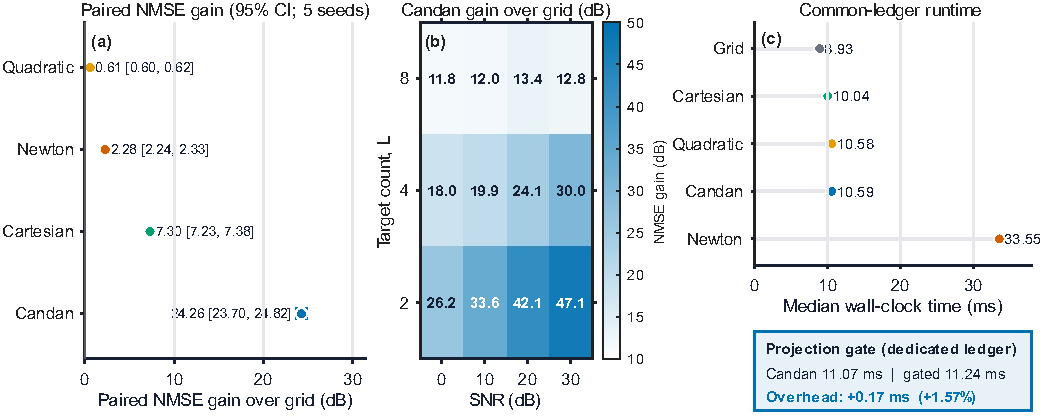
\includegraphics[width=0.96\textwidth]{tsp_local_family.pdf}
  \caption{Matched-scene evidence on the common 1200-tensor campaign. (a) Paired measurement-NMSE gain over FFT top-$L$ plus joint LS for four local refinements; dots and bars are the mean and 95\% interval over five seed means (higher is better). (b) Candan gain across SNR and target count; every displayed condition is positive. (c) Common-ledger median end-to-end runtime, with a separate dedicated-implementation inset showing that fitted-energy selection adds 0.17 ms (1.57\%) to local Candan.}
  \label{fig:local_family}
\end{figure*}

\subsection{Full-Offset and Independent MATLAB Replication}
\label{sec:full_offset}

When every fractional coordinate is uniform on the complete $[-0.49,0.49]$ interval, the local Candan stage reaches $-18.05$ dB from a $-3.60$ dB grid baseline, a 14.45 dB gain. Projection selection returns Candan throughout these 1200 scenes. Its all-axis half-bin rate is 0.652 versus 0.520 for grid. The same scenes give 6.62 dB for Cartesian refinement and 1.43 dB for quadratic interpolation, confirming that the complex ratio retains a substantial advantage beyond the narrower common offset range.

An independent MATLAB implementation separately generates 1200 scenes, reads the complex FFT triplets, applies Eq.~\eqref{eq:candan_update}, and performs joint LS. It obtains 23.36 dB mean gain with a five-seed 95\% interval of $[22.67,24.06]$ dB; all 1200 updates improve the grid reconstruction. This independent implementation verifies the accuracy scale with a different portable random generator.

\subsection{Projection-Selected Candan on CDL Channels}
\label{sec:reliability}

The projection rule returns Candan in 82.0\% of the 9000 tests, retaining 92.9\% of beneficial updates and filtering 75.7\% of harmful updates. Aggregate gain rises from 5.138 to 5.280 dB. The paired seed-level increment is 0.141 dB with a 95\% interval of $[0.097,0.186]$ dB.

Table~\ref{tab:candan_gate_profiles} shows the profile behavior directly. CDL-A and CDL-C retain their 10.22 and 4.91 dB gains, while CDL-D rises from 0.284 to 0.712 dB. The paired D increment is 0.428 dB with interval $[0.321,0.536]$ dB. The return rate changes from 99.8\% on CDL-A to 52.2\% on CDL-D under the same fitted-energy rule.

\begin{table}[!t]
\centering
\caption{Gain relative to grid for calibration-free projection selection on five CDL test seeds. Intervals are paired over seed means.}
\label{tab:candan_gate_profiles}
\scriptsize
\setlength{\tabcolsep}{2.5pt}
\begin{tabular}{lrrrr}
\toprule
Profile & Candan & Proj.-selected & Increment [95\%] & Return \\
 & (dB) & (dB) & (dB) & (\%) \\
\midrule
CDL-A & 10.223 & 10.220 & $-0.003\,[-0.009,0.002]$ & 99.8 \\
CDL-C & 4.907 & 4.907 & $-0.000\,[-0.033,0.032]$ & 93.9 \\
CDL-D & 0.284 & 0.712 & $0.428\,[0.321,0.536]$ & 52.2 \\
All & 5.138 & 5.280 & $0.141\,[0.097,0.186]$ & 82.0 \\
\bottomrule
\end{tabular}
\end{table}


The physical-parameter replay uses the same 9000 decisions and reproduces every channel-NMSE value exactly. Aggregate delay RMSE decreases from 428.45 ns for grid to 414.13 ns for Candan and 413.52 ns after projection selection. Joint quarter-bin accuracy rises from 7.46\% to 19.21\% and 18.84\%, while joint tenth-bin accuracy rises from 4.35\% to 9.12\% and 9.36\%. These results connect the channel-domain gain to lower delay error and higher joint-coordinate accuracy.

\subsection{Controlled Separation and Near--Far Stress}
\label{sec:stress}

The $L=4$ campaign inserts one controlled pair at 0.25, 0.5, 1, or 2 bins, cycles the pair across the three axes, and sets its dynamic range to 0, 10, or 20 dB. Local Candan gain is positive in all 48 SNR-resolved cells: the average is 10.46 dB with a five-seed interval of $[9.91,11.01]$ dB, and the minimum cell is 6.29 dB with interval $[4.44,8.15]$ dB. Projection selection returns Candan throughout the campaign. Per-component all-axis half-bin accuracy rises from 51.5\% for the grid coordinates to 68.9\%. Figure~\ref{fig:stress} shows how separation and dynamic range affect grid accuracy, Candan accuracy, designated-pair recovery, and reconstruction gain.

\begin{figure*}[t]
  \centering
  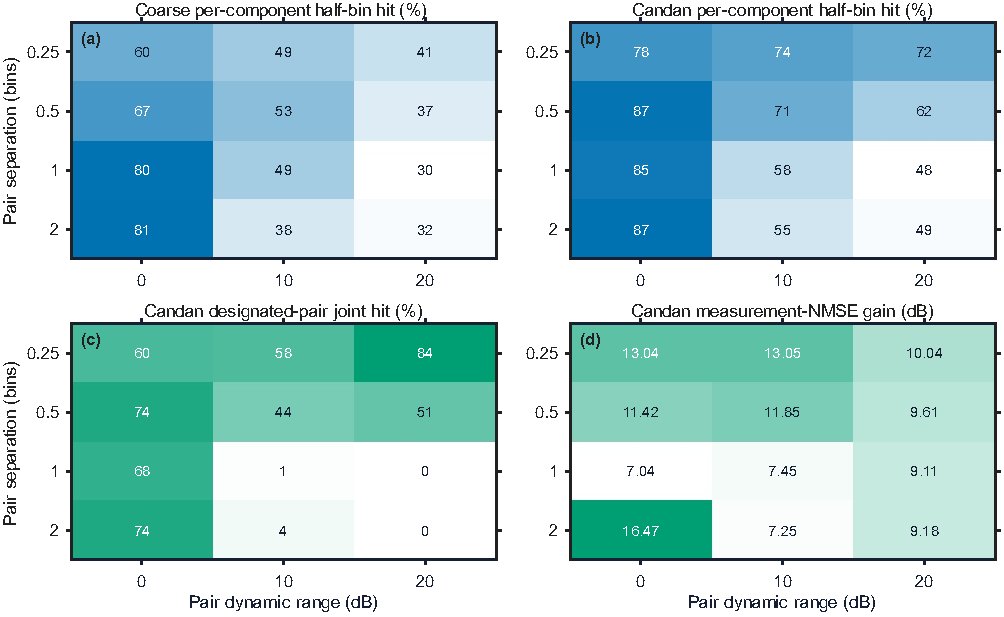
\includegraphics[width=0.88\textwidth]{tsp_stress_mechanism.pdf}
  \caption{Controlled separation/near--far evidence averaged over four SNRs, with 100 test scenes and five seed means per displayed cell. Panels (a) and (b) share a 0--100\% scale for direct comparison of grid and Candan per-component all-axis half-bin rates; (c) reports designated-pair joint recovery; and (d) reports measurement-NMSE gain over grid. All displayed reconstruction gains are positive.}
  \label{fig:stress}
\end{figure*}

\section{Discussion}

The results identify a consistent operating point between an integer-grid FFT estimator and iterative continuous recovery. Candan uses the complex peak triplets already exposed by the FFT and reaches 24.26 dB gain on the common tensor model and 14.45 dB over the complete fractional-bin interval. The optimized projection-selected implementation takes 11.24 ms, and the independent MATLAB implementation reproduces the same accuracy scale.

The theory characterizes the triplet perturbations after FFT neighborhood selection. Proposition~1 removes the non-updated tensor axes from every isolated quotient exactly. Proposition~2 then exposes how separation, dynamic range, sparsity, aperture, and SNR perturb that scalar problem, while Corollary~1 propagates coordinate error to joint LS. The controlled separation--near--far campaign complements this analysis by varying the main interference terms and retaining positive Candan gain in every tested cell.

The controlled-pair campaign shows that reconstruction gains persist across the tested separation and near--far conditions. Its one-shot FFT top-$L$ interface refines the selected neighborhoods as a group, so reconstruction NMSE and strict distinct-pair recovery describe complementary aspects of performance when leakage peaks share a physical component.

Projection selection adds a scene-level reliability layer after all coordinates and amplitudes have interacted. The fitted-energy rule preserves the large A/C gains and improves the D profile, yielding a statistically resolved 0.141 dB aggregate increment. This division of labor is simple: the complex ratio supplies a closed-form local coordinate, joint LS reconciles the selected components, and fitted energy decides which complete reconstruction is returned.

The fitted-energy decision directly targets received-subspace reconstruction, while the physical replay evaluates the returned components. Lower aggregate delay RMSE and more than doubled tenth- and quarter-bin joint hit rates show that projection selection preserves the parameter benefit of Candan refinement while strengthening channel reconstruction.

\section{Conclusion}

Projection-selected multidimensional Candan refinement turns an FFT top-$L$ support list into a continuous coordinate-and-amplitude estimate using $3DL$ complex samples, joint LS, and one fitted-energy decision. Exact separable triplet reduction, an interference-and-noise quotient bound after neighborhood selection, and a steering-Jacobian result connect Fourier geometry to the local update and joint fit. The Candan stage provides 24.26 dB common-scene gain, 14.45 dB over the full fractional-bin range, and positive gain in all 48 controlled stress cells. The complete estimator takes 11.24 ms, matches the Candan result throughout those synthetic campaigns, and raises CDL aggregate gain to 5.28 dB and CDL-D gain to 0.71 dB while improving aggregate physical-parameter metrics. These results establish a reproducible closed-form refinement path for FFT-selected tensor neighborhoods.


\section*{Reproducible Research}
The generators, evaluation scripts, aggregate tables, independent MATLAB implementation, and MATLAB figure sources are available at \url{https://github.com/Adonis-0311/OFDM-MIMO-Project}.

\section*{Acknowledgment}
This work received no external funding. AI-assisted tools were used solely for language polishing. The authors independently developed and verified all technical content, numerical results, figures, and conclusions and take full responsibility for the article.

\bibliographystyle{IEEEtran}
\IEEEtriggeratref{20}
\bibliography{../../../02_literature_and_refs/v2_3r_references,tsp_additions}

\end{document}
